
\section{Agent Controller}

The agent controller is designed specifically to be able to accommodate
all types of APL. This means that a lot of special care had to be
taken in order for us to impose as few restrictions as possible. This
section will focus on the different designs we went through and why
we eventually landed on the design we have now.

\begin{figure}
\begin{centering}
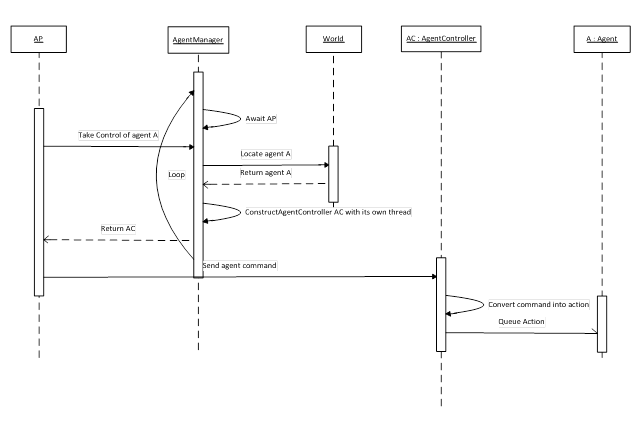
\includegraphics[width=0.7\textwidth]{ImplementationAgentControllerSequenceDiagram}
\par\end{centering}

\caption{This image details exactly how an \texttt{AgentManager} Processes
incoming requests from an outside AP \label{fig:ImplementationAgentControllerSequenceDiagram}}
\end{figure}



\subsection*{Explanation}

The \texttt{AgentManager} is designed to run separately from the engine\textquoteright{}s
model thread, which means it has the ability to take all the time
needed to properly connect to an outside AP, same goes for the \texttt{AgentController}.
This means that when an \texttt{AgentManager} generates a new \texttt{AgentController}
to be used by the AP, it also generates a new thread which the \texttt{AgentController}
is executed on. In the System Features section we covered how \texttt{AgentController}s
are used. Here we will elaborate on the exact process. In fig. \ref{fig:ImplementationAgentControllerSequenceDiagram},
a sequence diagram is shown that looks familiar to the one shown in
the system features. However there are a few key differences. First,
this sequence diagram shows the complete life cycle of an \texttt{AgentManager},
since the \texttt{AgentManager} is running on its own thread it does
not care about blocking until work needs to be done and the only kind
of work it is responsible for is ensure that \texttt{AgentController}s
are generated for APs in need of them. Second, it also details that
\texttt{AgentController}s are in fact generated by the \texttt{AgentManager}
with its own thread.


\subsection*{Considerations}

The \texttt{AgentManager} went through many design iterations in order
to arrive at its present state. Originally, the \texttt{AgentManager}
was called \texttt{AgentServer}. The reason was that for another language
to interface with the language of the engine -- C\# -- there must
be a universal way of connecting the two languages. A way in which
practically no languages was prohibited from interacting, and as we
thought such a way could only be achieved through a TCP connecting
since the protocol for TPC connections is very old and as such usable
in most languages by far. While it is true that probably almost all
languages do require a TCP connecting in order for them to work with
our engine, it is not true for languages that the engine understand,
considering that all the .NET platform languages works together very
well. For example, you could use the functional programming language
F\#, which also runs on the .NET platform. As such, if we imposed
that all \texttt{AgentManager}s are \texttt{AgentServer}s, it would
be required to setup a server just for using a language which the
engine already understands. \texttt{\emph{{[}Consider rewriting paragraph
from another standpoint: AgentManager is more general, less restrictive
than AgentServer{]}}}


\subsection*{Summary}

\texttt{AgentManager} and \texttt{AgentController} is designed as
a framework for making an interface between an APL and the engine.
They are intentionally made very lightweight so that they do not prohibit
the any special requirements of any given APL.
